%%
%% This is file `sample-sigconf.tex',
%% generated with the docstrip utility.
%%
%% The original source files were:
%%
%% samples.dtx  (with options: `sigconf')
%% 
%% IMPORTANT NOTICE:
%% 
%% For the copyright see the source file.
%% 
%% Any modified versions of this file must be renamed
%% with new filenames distinct from sample-sigconf.tex.
%% 
%% For distribution of the original source see the terms
%% for copying and modification in the file samples.dtx.
%% 
%% This generated file may be distributed as long as the
%% original source files, as listed above, are part of the
%% same distribution. (The sources need not necessarily be
%% in the same archive or directory.)
%%
%% The first command in your LaTeX source must be the \documentclass command.
\documentclass[sigconf]{acmart}

%%
%% \BibTeX command to typeset BibTeX logo in the docs
\AtBeginDocument{%
  \providecommand\BibTeX{{%
    \normalfont B\kern-0.5em{\scshape i\kern-0.25em b}\kern-0.8em\TeX}}}

%% Rights management information.  This information is sent to you
%% when you complete the rights form.  These commands have SAMPLE
%% values in them; it is your responsibility as an author to replace
%% the commands and values with those provided to you when you
%% complete the rights form.
\setcopyright{acmcopyright}
\copyrightyear{2018}
\acmYear{2018}
\acmDOI{10.1145/1122445.1122456}

%% These commands are for a PROCEEDINGS abstract or paper.
\acmConference[Woodstock '18]{Woodstock '18: ACM Symposium on Neural
  Gaze Detection}{June 03--05, 2018}{Woodstock, NY}
\acmBooktitle{Woodstock '18: ACM Symposium on Neural Gaze Detection,
  June 03--05, 2018, Woodstock, NY}
\acmPrice{15.00}
\acmISBN{978-1-4503-XXXX-X/18/06}


%%
%% Submission ID.
%% Use this when submitting an article to a sponsored event. You'll
%% receive a unique submission ID from the organizers
%% of the event, and this ID should be used as the parameter to this command.
%%\acmSubmissionID{123-A56-BU3}

%%
%% The majority of ACM publications use numbered citations and
%% references.  The command \citestyle{authoryear} switches to the
%% "author year" style.
%%
%% If you are preparing content for an event
%% sponsored by ACM SIGGRAPH, you must use the "author year" style of
%% citations and references.
%% Uncommenting
%% the next command will enable that style.
%%\citestyle{acmauthoryear}

\usepackage{graphicx}

%%
%% end of the preamble, start of the body of the document source.
\begin{document}


\title{Cybercrime and Online Video Games}

\author{Emilio Lopez}
\affiliation{%
  \institution{Case Western Reserve University}
  \streetaddress{10900 Euclid Ave}
  \city{Cleveland}
  \country{Ohio}}
\email{eil11@case.edu}

\author{Cameron Hochberg}
\affiliation{%
  \institution{Case Western Reserve University}
  \streetaddress{10900 Euclid Ave}
  \city{Cleveland}
  \country{Ohio}}
\email{clh137@case.edu}

\author{Michael Silverman}
\affiliation{%
  \institution{Case Western Reserve University}
  \streetaddress{10900 Euclid Ave}
  \city{Cleveland}
  \country{Ohio}}
\email{mhs126@case.edu}

\author{Anthony Smith}
\affiliation{%
  \institution{Case Western Reserve University}
  \streetaddress{10900 Euclid Ave}
  \city{Cleveland}
  \country{Ohio}}
\email{aas182@case.edu}

%% By default, the full list of authors will be used in the page
%% headers. Often, this list is too long, and will overlap
%% other information printed in the page headers. This command allows
%% the author to define a more concise list
%% of authors' names for this purpose.
\renewcommand{\shortauthors}{Lopez, Hochberg, Silverman and Smith}

%%
%% The abstract is a short summary of the work to be presented in the
%% article.
\begin{abstract}
  [REWRITE THIS AT END]
  The growth of online video games has yielded a vast underground economy of
  criminals who sell exploits and credentials to give gamers unfair advantages
  in the games. This paper studies the sale of ``crimeware'' connected to
  the Epic Games' ``Fortnite: Battle Royale'' video game. The authors created 
  a webscraping tool to collect large amounts of data from a hacker forum to 
  analyze key distributers in the economy.
\end{abstract}

%%
%% The code below is generated by the tool at http://dl.acm.org/ccs.cfm.
%% Please copy and paste the code instead of the example below.
%%
% i never got this to work
\begin{CCSXML}
<ccs2012>
 <concept>
  <concept_id>10010520.10010553.10010562</concept_id>
  <concept_desc>Computer systems organization~Embedded systems</concept_desc>
  <concept_significance>500</concept_significance>
 </concept>
 <concept>
  <concept_id>10010520.10010575.10010755</concept_id>
  <concept_desc>Computer systems organization~Redundancy</concept_desc>
  <concept_significance>300</concept_significance>
 </concept>
 <concept>
  <concept_id>10010520.10010553.10010554</concept_id>
  <concept_desc>Computer systems organization~Robotics</concept_desc>
  <concept_significance>100</concept_significance>
 </concept>
 <concept>
  <concept_id>10003033.10003083.10003095</concept_id>
  <concept_desc>Networks~Network reliability</concept_desc>
  <concept_significance>100</concept_significance>
 </concept>
</ccs2012>
\end{CCSXML}

\ccsdesc[500]{Computer systems organization~Embedded systems}
\ccsdesc[300]{Computer systems organization~Redundancy}
\ccsdesc{Computer systems organization~Robotics}
\ccsdesc[100]{Networks~Network reliability}

%%
%% Keywords. The author(s) should pick words that accurately describe
%% the work being presented. Separate the keywords with commas.
\keywords{web scraping, sentiment analysis, cybercrime, video games}

%%
%% This command processes the author and affiliation and title
%% information and builds the first part of the formatted document.
\maketitle

\section{Introduction}

Since their inception decades ago, video games have become hugely preavalent in
society. Millions of people play video games as a hobby, and their demographics
span all age groups, ethnicities, and socioeconomic class. In particular, online
multiplayer video games have become hugely popular. Many of these games are 
highly competitive, and there any many players who look for unfair advantages in
the form of video game cheats. Video game cheats give the player abilities to 
to outperform their opponents. This competitive milieu has led to the
development of thriving marketplaces and economies devoted to creation and 
distribution of video game cheats. Online hacker forums are places where 
interested parties can sell, discuss, and review video game cheats. However, 
these vendors not only sell cheats but also online video game accounts. These
are especially desirable to perons who have been forbidden from playing an 
online game by the developers - usually for cheating or other malicious
behavior. Often, these accounts are stolen from innocent users and sold to 
malicious actors. Many of the players of online video games are 
children, and thus they are often the victims of account theft. This paper 
explores the crimware economy devoted to "Fortnite: Battle Royale."

\section{Background}

\subsection{Fortnite: Battle Royale}
Developed by Epic Games, "Fortnite: Battle Royale" or "Fortnite" is a 
third-person shooter and battle royale online video game. The player must
utilize a diverse arsenal of weapons to defeat 99 other human opponents and 
claim victory. 

\subsection{Hack Forums}
There exist many forums on the Internet for persons interested in computer
hacking, but one the most visited is Hack Forums (hackforums.net). Ranked
second in top sites for "hacking" % (https://www.alexa.com/topsites/category/Top/Computers/Hacking), Hack Forums has several discussion boards
on topics ranging from social engineering techniques to Internet-of-Things 
exploits. On Hack Forums, users make accounts to use the community forums:
posting, searching, and even browsing requires an account to be registered.
Users also can give feedback on each other. For example, a user with
a high feedback score will be regarded as more trustworthy. Often, these users
gain repute by participating in discussion or selling a legitimate product or 
service. Users can also privately message each other, without having to use
another service like email. Due to Hack Forums' prominence and enablement of 
cybercrime, it merited our scrutiny to examine its contribution to cybercrime
in the video game space. 

\subsection{Web Scraping}
Web scraping refers to the process of extracting data from web pages, and the 
term typically implies the automation of this process. Data extracted from web
pages will then be parsed to be usable. Often, websites will not provide 
easily accessible data sets of the website content, which means that a 
web scraping program must be written to extract the relevant information from
the HTML present on the page. Given the sheer volume of information that must
be collected, the best action is to implement our own program to scrape data 
from Hack Forums.

\subsection{Sentiment Analysis}
One of our tasks was to analyze the intentions behind each comment, whether
they were criticizing the product or, on the contrary, if they were lauding
the product. For that, we decided to use a Python package provided by scikit-learn.org
We used 3 different machine learning techniques to classify each comment as
either positive or negative: Stochastic Gradient Descent (SGD), Naive Bayes, 
Support Vector machines (SVC). Each algorithm gives each comment a probability to be either positive or negative. We sum each algorithm's score and determine based on that score whether the comment is positive, negative or neutral.


\section{Crimeware}

\subsection{Video Game Cheats}

\subsubsection{Aimbots}
Aimbots are a sub set of game hacks. These reffer to scripts that run on the client side of the game 
and track things such as hit boxes of other players in the game and aim for you once activated. It is 
an easy kind of cheat to spot as it will usually result in unhuman reflexes or movement or such things 
as wall tracking where a player is aiming at you through a wall. Since they also track only specific 
areas, a statistical analysis of the areas where the player regularly hit his targets can reveal whether 
or not he was hacking. Normal humans can't aim at the same target over a long period of time and will
usually stay within one or two standard deviations of the mean for any given area. Someone who aimbots 
on the other hand will usually have one area that is way above the mean.

\subsubsection{Hacks}
There are several versions of this cheat but there is usually two types: a script that uses a bug from the
developer to allow the user to view more than he should be making walls transparent or "see-through"; 
another would be to make walls non solid objects allowing the player to shoot through walls or 
even hide in them. These hacks usually relly on the fact the FPS games in particular send 
only the raw positional information of players and let the player or client's 3D renderer to 
hide other players behind walls or through "fog of war". These can be turned off from the client 
side and thus make it look like the players are moving around what seams like an empty space. 
Obviously a completely empty map serves no purpose for the hacker as he couldn't navigate the map properly 
either. This third party software allows the user to only hide certain surfaces from its client 3D 
renderer so that the hacker may have an edge compared to other players.

\subsubsection{Nuking or artificial lag}
The sub genre of hacks, as its name suggests, consists of artificially generating lag between the 
client and the server in order to gain an advantage. In some games, hits aren't registered until 
the server registeres a hit. In this case, overloading the server with packets just enough to create lag
for every player on the server but not enough to cause the server to crash allows you to stall the game
enough for you to be able to win effortlessly in the next round.

\subsubsection{Code Injection}
"Code Injection is the general term for attack types which consist of injecting code that is then 
interpreted/executed by the application."\cite{codeinjection}
Usually these attacks are the result of poor data validation from input/output. Code Injection deffiers from
Command Injection in the sense that the attacker, in the case of Command Injection, is limited by what the API
has to offer; while Code Injection is only limited by the language used. The risk from Code Injection if that,
if the attack is successful, this can lead to loss of data, confidentiality and loss of availability.

\subsection{Account Sales}


\section{Method}

\subsection{Web Scraper Implementation}
We opted to implement our web scraping program in the Python 3 programming
language. Given the time constraints of the project, we found that Python
matched our needs well given its rapid development time. In addition, the 
external library support of Python was deemed essential in traversing
Hack Forums and extracting the data. We also used Selenium web automation tool
and its relevant Python bindings. For Python, we also used the "Requests" and 
"BeautifulSoup" libraries. "Requests" simplifies the creation of HTTP requests 
to obtain web content, and "BeautifulSoup" is an HTML parser which assists
in unraveling the web page content to extract. Finally, to actually create
the requisite Excel file, we used the OpenPyXL library to generate and
populate the file. 

Since the program's scraping is based on the website's specific content and 
design (e.g., names of tag classes and id attributes in the page HTML), the web
scraper can only be used for Hack Forums. Hack Forums provided some unique
challenges for our scraping. For example, the website seems to heavily rely
on the PHP programming language. For searching the forum threads, this is 
troublesome, because the search itself is not a simple web endpoint where the 
search term can be replaced. This design decision requires the use of Selenium
to "click" buttons and enter search terms into the website's forms. For each
page of search results, the URL for the thread is acquired along with the 
original poster, number of replies, and other relevant information. With the 
URL for a thread, the comment pages are requested and the relevant information
per comment is scraped from each page for the thread.

After all the is collected from a search, the data is written to an Excel file
which contains all the results. With all the data aggregated, manual data
analysis can begin.


[DISCUSS OUR TECHNIQUE OF DATA ANALYSIS - i.e, sentiment analyze all, then manually confirm other details]

However, the data analysis for sentiment does not always apply to the comment.
For example, if the comment is actually a question or a request to receive a 
private message, then AI sentiment analysis of the comment is likely irrelevant.
Therefore, the comments must be analyzed for different criteria. For example, 
if the comment is actually a user "bumping" the thread, then it should be 
discarded. It was not feasible for us to develop an AI solution to accurately
categorize comments in each possible scenario, so we have chosen to automate
the collection of data but manually classify it.

\section{Results}

% The title of your work should use capital letters appropriately -
% \url{https://capitalizemytitle.com/} has useful rules for
% capitalization. Use the {\verb|title|} command to define the title of
% your work. If your work has a subtitle, define it with the
% {\verb|subtitle|} command.  Do not insert line breaks in your title.

% If your title is lengthy, you must define a short version to be used
% in the page headers, to prevent overlapping text. The \verb|title|
% command has a ``short title'' parameter:
% \begin{verbatim}
%   \title[short title]{full title}
% \end{verbatim}

% Above was too helpful to uncomment
[RAW RESULTS DATA, THEN REFINED DATA]
[TABLES WOULD BE HELPFUL HERE]

\subsection{Key Players}
In the context of our project, the key players in the Fortnite hacker forums are those who have the most threads and/or comments under their names. We defined a user as a key player if they posted more than one thread or more than fifty comments from our 104 threads and 7932 comments. We determined these metrics by manually analyzing the comments and threads and determining who were the minority of more active users. These active user threads will usually take the form of either crimeware or CaaS with the poster selling to whoever can pay with some supposedly “legal” methods scattered throughout. Some of the more popular services are account selling, radar hacks, aimbot hacks and cheaper V-Bucks. Below are two pie charts depicting the thread and comment counts with the labels identifying the greater contributors.


\begin{figure}
\centering
\begin{subfigure}{.5\textwidth}
 	\centering
	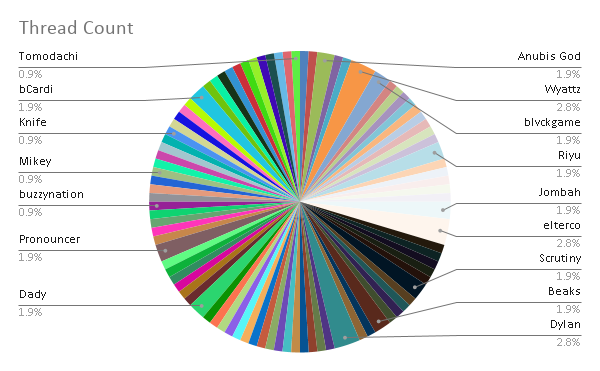
\includegraphics[width = .4\linewidth]{ThreadCount.png}
	\caption{Thread Count}
\end{subfigure}
\begin{subfigure}{.5\textwidth}
 	\centering
	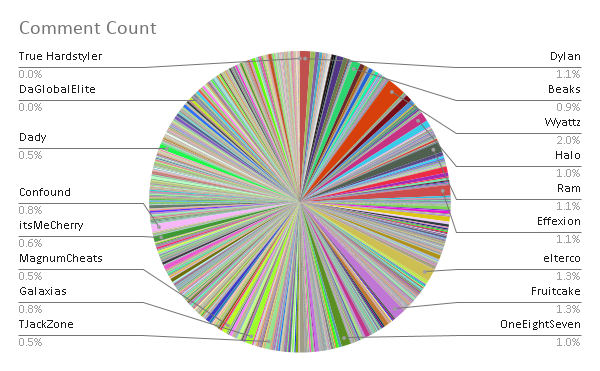
\includegraphics[width=.4\linewidth]{CommentCount.png}
	\caption{Comment Count}
\end{subfigure}
\caption{Thread and Comment Pie Charts}
\end{figure}


\subsubsection{Wyattz}
Wyattz can be considered the most active user on the Fortnite hacker forums being tied for the most threads at three and having the most comments at 162. Wyattz is also a veteran member of hackforums.net and appears to be a trusted source of “legal” software and methods. His Fortnite posts revolve around making money playing Fortnite using what he claims to be a legal method. Since we were unable to access his method we could not determine its legality but his customers have commented back with general satisfaction. The other factor that makes Wyattz interesting is his number of comments. These comments were not made on other threads but on his own. His comments are either responses to other user’s comments or simply declarations that he is online and ready to talk. Wyattz places a lot of effort into his work on hackerforum so even though his comments rarely range outside his own threads and his product is not explicitly illegal, he is still a major player worth looking at.

\subsubsection{Jombah}
Jombah is also considered a key player on the Fortnite hacker forums even though he is on the lower end of the thread and comment counts with only two threads and 43 comments. He still passes the threshold for being a key player but the reason he is being focused on is due to his product. Jombah sells Fortnite accounts which is one of the crimewares we are focusing on. Jombah’s products are “premium” accounts which he appears to sell for a relatively cheap price as compared to other sellers though unlike some other sellers he does not offer custom accounts that a buyer can specify. Jombah is also a decently active user on hackerforum.net though not as active as Wyattz or as well liked by his customers. Jombah’s relevance lies not with his stellar service but with the product he provides.

\subsubsection{Dylan}
The last key player we will feature is probably the most important figure in the overall Fortnite hackforum community, though that is not saying much. Dylan provides the cheats for users such as radar and silencers. His presentation and communication with clients is professionally done and there are very few complaints regarding his product. While this is important for Dylan’s hierarchy as a key player, what is most important about him is that he interacts with other Fortnite posters. While analyzing threads and comments, we noticed that very few posters comment beyond their threads. There is little to no communication among the Fortnite hackforum community. Dylan is the exception to the rule. He comments on other threads whether he is providing explanations of services, vouching for others or shooting down fraudulent products. Dylan is not the most active user in his community, but nobody is as far reaching making him the most important key player in this community.

\subsection{Key Players Conclusion}
After analyzing the comments and threads we formed a decent understanding of the hackforum Fortnite community. The community doesn’t appear to revolve around any given person or group with many independent people providing products and/or services to Fortnite players. Even the most active figures in the community don’t communicate with each other in general. The Fortnite threads almost cannot be considered a community, more like a loose collection of people with similar ideas. This makes the key players less important as nobody has control over any aspect of the community.

%[A table would be a nice addition here]
%[DISCUSS THE DIFFERENT KEY MEMBERS OF THE COMMUNITY]
%[WHICH CHEATS ARE MOST POPULAR]

\section{Solutions}
\subsection{Video Game Cheats}
\subsubsection{Mirrored server design}
The general idea for this is that all client functionality runs either solely on the server
or alternatively, it runs synchronously between the client and a miror of the game server. This way,
the state of the game is continously validated where the miror server uses the exact same inputs received
to validate the results from the client game. If there is ever a discrepency, the client's game session resets 
and thus prevents cheating by reseting the game state to the last valid state of the game. One problem that isn't so
common is that this method requires a lot of bandwidth, storage and memory but nowadays, most of those concerns are minimal.

\subsubsection{Pattern Detection/Analyze performance}
This is a common way of detecting cheats for most online games since it rarely affects players direcly due to its 
none invasive nature. Like normal anti virus software, some program in the game
will scan the hard drive to find any know cheat software or cheat codes. Another is that it will analyze the statistical
data from the player. For example, you might want to see how often a player is able to hit a certain part of the hitboxes
of other players. If there is a statistical different greater than the expected standard deviation, there is a high chance
that the player is cheating. However, thsi method also leads to false positive/negative. Very highly skilled players may
get flagged as cheaters because of how good they are, while others may use cheats but in areas that aren't verified by the
statistical data and thus be flagged as regular player.

\subsubsection{Player Supervision}
This is a more intrusive method of detection as it requires someone monitoring the player. Obviously, it is impossible
to monitor every single player in the game but this method can be used in conjonction with Pattern detection. If a player
is flagged, he doesn't have to be banned just yet, that could mean that someone can start reviewing that player's 
gameplay and decide for himself whether or not that player is cheating or not. Some games have implemented player 
supervision by allowing the community to send reports of disruptive behavior or suspected cheating. 
Reports can include data such as screenshots, videos, and chatlogs that are then sent to the administrators of the gamef
for review. If the player reported happens to be cheating any form of punishment can be dispensed.

\subsection{Account Theft}
% [MFA (already in Fortnite) but suggest mandating it]
Given the prominence of account theft and sales, we propose that Fortnite -
and other online video games like it - mandate the use of multi-factor
authentication (MFA) in combination with username and password credentials to
secure accounts. Epic Games has already implemented an MFA tool for players to 
use to protect their accounts, and the game incentivizes players to use it;
however, we argue that optional usage of MFA is insufficient, and that online 
video game developers should require the usage of MFA as part of accessing one's
account. Additionally, we suggest that video game developers create their own 
solution instead of relying on a simple SMS numerical code. SMS messages can be 
intercepted, and an attacker can actually acquire the code for login. However,
a robust, novel implementation can likely thwart the majority of hackers and 
provide for the safety of a user's account.

% [FIND STATS OF HOW IT REDUCES BREACHES]
% https://security.googleblog.com/2019/05/new-research-how-effective-is-basic.html

\section{Conclusion}
[CONCLUDE]
[ALSO DISCUSS WHAT WE LEARNED (I think she wants that...)]


% Information on how to make tables

% \section{Tables}

% The ``\verb|acmart|'' document class includes the ``\verb|booktabs|''
% package --- \url{https://ctan.org/pkg/booktabs} --- for preparing
% high-quality tables.

% Table captions are placed {\itshape above} the table.

% Because tables cannot be split across pages, the best placement for
% them is typically the top of the page nearest their initial cite.  To
% ensure this proper ``floating'' placement of tables, use the
% environment \textbf{table} to enclose the table's contents and the
% table caption.  The contents of the table itself must go in the
% \textbf{tabular} environment, to be aligned properly in rows and
% columns, with the desired horizontal and vertical rules.  Again,
% detailed instructions on \textbf{tabular} material are found in the
% \textit{\LaTeX\ User's Guide}.

% Immediately following this sentence is the point at which
% Table~\ref{tab:freq} is included in the input file; compare the
% placement of the table here with the table in the printed output of
% this document.

% \begin{table}
%   \caption{Frequency of Special Characters}
%   \label{tab:freq}
%   \begin{tabular}{ccl}
%     \toprule
%     Non-English or Math&Frequency&Comments\\
%     \midrule
%     \O & 1 in 1,000& For Swedish names\\
%     $\pi$ & 1 in 5& Common in math\\
%     \$ & 4 in 5 & Used in business\\
%     $\Psi^2_1$ & 1 in 40,000& Unexplained usage\\
%   \bottomrule
% \end{tabular}
% \end{table}

% To set a wider table, which takes up the whole width of the page's
% live area, use the environment \textbf{table*} to enclose the table's
% contents and the table caption.  As with a single-column table, this
% wide table will ``float'' to a location deemed more
% desirable. Immediately following this sentence is the point at which
% Table~\ref{tab:commands} is included in the input file; again, it is
% instructive to compare the placement of the table here with the table
% in the printed output of this document.

% \begin{table*}
%   \caption{Some Typical Commands}
%   \label{tab:commands}
%   \begin{tabular}{ccl}
%     \toprule
%     Command &A Number & Comments\\
%     \midrule
%     \texttt{{\char'134}author} & 100& Author \\
%     \texttt{{\char'134}table}& 300 & For tables\\
%     \texttt{{\char'134}table*}& 400& For wider tables\\
%     \bottomrule
%   \end{tabular}
% \end{table*}

% In case we want to add figures to our paper
% \section{Figures}

% The ``\verb|figure|'' environment should be used for figures. One or
% more images can be placed within a figure. If your figure contains
% third-party material, you must clearly identify it as such, as shown
% in the example below.
% % \begin{figure}[h]
% %   \centering
% %   \includegraphics[width=\linewidth]{sample-franklin}
% %   \caption{1907 Franklin Model D roadster. Photograph by Harris \&
% %     Ewing, Inc. [Public domain], via Wikimedia
% %     Commons. (\url{https://goo.gl/VLCRBB}).}
% %   \Description{The 1907 Franklin Model D roadster.}
% % \end{figure}

% Your figures should contain a caption which describes the figure to
% the reader. Figure captions go below the figure. Your figures should
% {\bfseries also} include a description suitable for screen readers, to
% assist the visually-challenged to better understand your work.

% Figure captions are placed {\itshape below} the figure.

% \subsection{The ``Teaser Figure''}

% A ``teaser figure'' is an image, or set of images in one figure, that
% are placed after all author and affiliation information, and before
% the body of the article, spanning the page. If you wish to have such a
% figure in your article, place the command immediately before the
% \verb|\maketitle| command:
% \begin{verbatim}
%   \begin{teaserfigure}
%     \includegraphics[width=\textwidth]{sampleteaser}
%     \caption{figure caption}
%     \Description{figure description}
%   \end{teaserfigure}
% \end{verbatim}

% \section{Citations and Bibliographies}

% The use of \BibTeX\ for the preparation and formatting of one's
% references is strongly recommended. Authors' names should be complete
% --- use full first names (``Donald E. Knuth'') not initials
% (``D. E. Knuth'') --- and the salient identifying features of a
% reference should be included: title, year, volume, number, pages,
% article DOI, etc.

% The bibliography is included in your source document with these two
% commands, placed just before the \verb|\end{document}| command:
% \begin{verbatim}
%   \bibliographystyle{ACM-Reference-Format}
%   \bibliography{bibfile}
% \end{verbatim}
% where ``\verb|bibfile|'' is the name, without the ``\verb|.bib|''
% suffix, of the \BibTeX\ file.

% Citations and references are numbered by default. A small number of
% ACM publications have citations and references formatted in the
% ``author year'' style; for these exceptions, please include this
% command in the {\bfseries preamble} (before
% ``\verb|\begin{document}|'') of your \LaTeX\ source:
% \begin{verbatim}
%   \citestyle{acmauthoryear}
% \end{verbatim}

%   Some examples.  A paginated journal article \cite{Abril07}, an
%   enumerated journal article \cite{Cohen07}, a reference to an entire
%   issue \cite{JCohen96}, a monograph (whole book) \cite{Kosiur01}, a
%   monograph/whole book in a series (see 2a in spec. document)
%   \cite{Harel79}, a divisible-book such as an anthology or compilation
%   \cite{Editor00} followed by the same example, however we only output
%   the series if the volume number is given \cite{Editor00a} (so
%   Editor00a's series should NOT be present since it has no vol. no.),
%   a chapter in a divisible book \cite{Spector90}, a chapter in a
%   divisible book in a series \cite{Douglass98}, a multi-volume work as
%   book \cite{Knuth97}, an article in a proceedings (of a conference,
%   symposium, workshop for example) (paginated proceedings article)
%   \cite{Andler79}, a proceedings article with all possible elements
%   \cite{Smith10}, an example of an enumerated proceedings article
%   \cite{VanGundy07}, an informally published work \cite{Harel78}, a
%   doctoral dissertation \cite{Clarkson85}, a master's thesis:
%   \cite{anisi03}, an online document / world wide web resource
%   \cite{Thornburg01, Ablamowicz07, Poker06}, a video game (Case 1)
%   \cite{Obama08} and (Case 2) \cite{Novak03} and \cite{Lee05} and
%   (Case 3) a patent \cite{JoeScientist001}, work accepted for
%   publication \cite{rous08}, 'YYYYb'-test for prolific author
%   \cite{SaeediMEJ10} and \cite{SaeediJETC10}. Other cites might
%   contain 'duplicate' DOI and URLs (some SIAM articles)
%   \cite{Kirschmer:2010:AEI:1958016.1958018}. Boris / Barbara Beeton:
%   multi-volume works as books \cite{MR781536} and \cite{MR781537}. A
%   couple of citations with DOIs:
%   \cite{2004:ITE:1009386.1010128,Kirschmer:2010:AEI:1958016.1958018}. Online
%   citations: \cite{TUGInstmem, Thornburg01, CTANacmart}. Artifacts:
%   \cite{R} and \cite{UMassCitations}.

\begin{acks}
  We would like to thank Professor Yanfang "Fanny" Ye of Case Western Reserve
  University for assisting us with the completion of our project. The guidance
  helped to refine the direction of our research and focus. With her assistance,
  we found a novel concept to explore.
\end{acks}

%%
%% The next two lines define the bibliography style to be used, and
%% the bibliography file.
\bibliographystyle{ACM-Reference-Format}
\bibliography{paper}{}

\end{document}
\endinput
%%
%% End of file `sample-sigconf.tex'.
